\subsection{Vorbereitung}

\begin{enumerate}
\item Zuerst wird ein Zylinderresonator zwischen Mikrofon und Lautsprecher platziert und anschließend mit dem Oszilloskop eine
Resonanz aufgenommen. Dazu wird der Lautsprecher an den einen Kanal des Oszilloskops angeschlossen, das Mikrofon an den
anderen. Von 6,75 kHz an wird die Frequenz nun immer weiter erhöht, bis eine zweite Resonanz gefunden wird.
Es werden Amplitudenspannung, Phasenverschiebung und Frequenz der beiden Resonanzen notiert.

Danach werden mehr und mehr Zylinderresonatoren zwischen Mikrofon und Lautsprecher platziert und die Messung wird
nach jedem neu hinzugefügten Zylinder wiederholt.

\item Im zweiten Teil der Vorbereitung wir das Oszilloskop im xy-Mode betrieben. Dann wird wieder genauso wie im ersten Teil
vorgegangen, wobei das Frequenzspektrum aufgenommen werden soll. Anschließend wird statt eines Oszilloskops ein PC zur
Aufnahme der Spektren genutzt.
\end{enumerate}

\begin{figure}
\centering
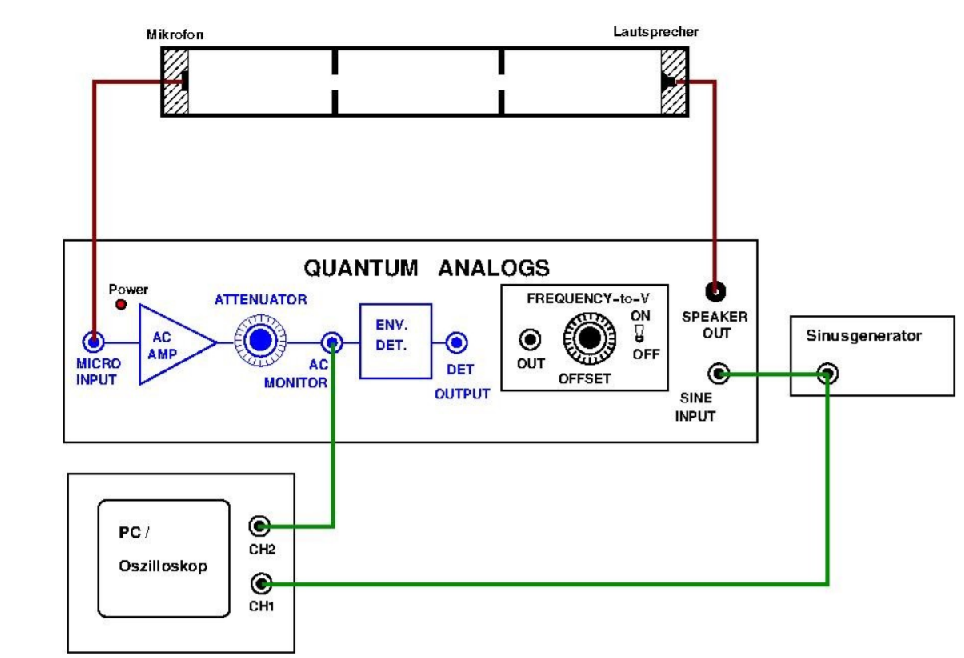
\includegraphics[width=0.6\textwidth]{versuchsaufbau.png}
\caption{Versuchsaufbau für den Versuch "Quantenanalogien". \cite[3]{anleitung}}
\label{fig:versuchsaufbau}
\end{figure}

\subsection{Wasserstoffatom}

In diesem Versuchsteil werden die beiden Kugelhälften mit dem eingebauten Mikrofon und Lautsprecher verwendet. Die beiden
Kugeln werden so aufeinandergesetzt, dass Lautsprecher und Mikrofon sich in einem 180°-Winkel gegenüberliegen. Anschließend
werden folgende Schritte durchgeführt:

\begin{enumerate}
\item Notieren der Resonanzfrequenzen für verschiedene Ordnungen und Beobachtung der Amplituden, Frequenzen und
Phasenverschiebungen (2-Kanal-Oszilloskop, Frequenzbereich 100Hz-10kHz).
\item Für den gleichen Frequenzbereich wird ein Frequenzspektrum mit dem PC aufgenommen.
\item Messung der Druckamplitude als Funktion des Winkels im Bereich 0°-180° für mindestens 3 Resonanzen (10°-Schrittweite).
\item Nacheinander werden Zwischenringe (3mm, 9mm und 3mm+9mm Dicke) zwischen die beiden Kugelhälften eingesetzt, die wieder im
180°-Winkel zueinander stehen und es wird die Aufspaltung der Resonanz bei den Frequenzen 2,1kHz und 2,3kHz vermessen.
\item Erneute Messung der Winkelabhängigkeit wie in Schritt 3 bei den Resonanzfrequenzen 2,1kHz und 2,3kHz. Dieses Mal mit
dem 9mm-Ring zwischen den Kugelhälften.
\end{enumerate}

\subsection{Wasserstoffmolekül}

Um das Wasserstoffmolekül zu simulieren, werden zwischen die beiden Halbkugeln mit dem Mikrofon und dem Lautsprecher zwei
weitere Halbkugeln mit Loch eingefügt. Es entstehen so zwei miteinander gekoppelte Kugelresonatoren. Lautsprecher und Mikrofon
sollten dabei wieder im 180°-Winkel zueinander stehen. Anschließend wird für verschiedene Blenden zwischen den beiden Kugeln
(ohne Blende, 5mm, 10mm, 15mm und 20mm) das Frequenzspektrum bei einer Resonanz von 2,3 kHz gemessen.

Dann wird eine beliebige Blendengröße ausgewählt und die Winkelabhängigkeit bei der Resonanz von 2,3 kHz gemessen.

\subsection{1-D Festkörper}

Es werden Aluminiumzylinder der Größe 50mm und Blenden der Größe 13mm ausgewählt. Anschließend wird das Frequenzspektrum für
einen Zylinder aufgenommen, danach für zwei Zylinder mit einer Blende dazwischen. Die Kette wird schrittweise verlängert
und vermessen bis sie zwölf Zylinder lang ist.

Danach wird einer der zwölf 50 mm langen Zylinder durch einen 75mm langen Zylinder ausgetauscht und es wird wieder das
Frequenzspektrum aufgenommen. Anschließend wird der 75mm-Zylinder durch zwei 12,5mm-Zylinder ersetzt und noch einmal wird das
Spektrum gemessen.

Zuletzt wird eine Kette aus zwölf 50mm langen Zylindern aufgebaut, die abwechselnd mit 13mm- und 16mm-Blenden gekoppelt sind.
